\documentclass[a4paper]{article}

%%%%%%%% CREATE DOCUMENT STRUCTURE %%%%%%%%
%% Language and font encodings
\usepackage[english]{babel}
\usepackage[utf8x]{inputenc}
\usepackage[T1]{fontenc}
%\usepackage{subfig}

%% Sets page size and margins
\usepackage[a4paper,top=3cm,bottom=2cm,left=2cm,right=2cm,marginparwidth=1.75cm]{geometry}

%% Useful packages
\usepackage{amsmath,amssymb}
\usepackage{graphicx}
\usepackage[colorinlistoftodos]{todonotes}
\usepackage[colorlinks=true, allcolors=blue]{hyperref}
\usepackage{caption}
\usepackage{subcaption}
\usepackage{sectsty}
\usepackage{apacite}
\usepackage{float}
\usepackage{titling} 
\usepackage{blindtext}
\usepackage[square,sort,comma,numbers]{natbib}
\usepackage[colorinlistoftodos]{todonotes}
\usepackage{xcolor}
\definecolor{darkgreen}{rgb}{0.0, 0.4, 0.0}
\usepackage{graphicx}
\newcommand{\norm}[1]{\left\lVert#1\right\rVert}
\DeclareMathOperator{\R}{\mathbb{R}}
\DeclareMathOperator{\E}{\mathbb{E}}

\usepackage{listings}
\usepackage{xcolor}

\definecolor{codegreen}{rgb}{0,0.6,0}
\definecolor{codegray}{rgb}{0.5,0.5,0.5}
\definecolor{codepurple}{rgb}{0.58,0,0.82}
\definecolor{backcolour}{rgb}{0.95,0.95,0.92}

\lstdefinestyle{mystyle}{
	backgroundcolor=\color{backcolour},   
	commentstyle=\color{codegreen},
	keywordstyle=\color{magenta},
	numberstyle=\tiny\color{codegray},
	stringstyle=\color{codepurple},
	basicstyle=\ttfamily\footnotesize,
	breakatwhitespace=false,         
	breaklines=true,                 
	captionpos=b,                    
	keepspaces=true,                 
	numbers=left,                    
	numbersep=5pt,                  
	showspaces=false,                
	showstringspaces=false,
	showtabs=false,                  
	tabsize=2
}

\lstset{style=mystyle}
 



%%%%%%%% DOCUMENT %%%%%%%%
\begin{document}

%%%% Title Page
\begin{titlepage}

\newcommand{\HRule}{\rule{\linewidth}{0.5mm}} 							% horizontal line and its thickness
\center 
 
 
% University


\includegraphics[width=0.15\textwidth]{images/kth_logo.png}\\[0.5cm] 	% University logo

\textsc{\LARGE KTH Royal Institute of Technology}\\[1cm]

% Document info
\textsc{\Large Deep Learning in Datascience}\\[0.2cm]
\textsc{\large DD2424}\\[1cm] 										% Course Code
\HRule \\[0.8cm]
{ \huge \bfseries Assignment 1}\\[0.7cm]								% Assignment
\HRule \\[2cm]
\large
\emph{Authors:}\\
Ali Banaei Mobarak Abadi\\[1.5cm]													% Author info
{\large \today}\\[5cm]

\vfill 
\end{titlepage}

%%\begin{abstract}
%%Your abstract.
%%\end{abstract}

%%%% SECTIONS
%% Section 1
\section{Assignment Report}
In this section, the results we can get by running the code are presented. For an explanation of the code and implementations, please see \autoref{sec:2}. Note that for the rest of this report, the available training data is divided into two parts, validation with a size of 5000 samples and the rest as training.

\subsection{Checking the gradients}

After implementing the code for the forward path and calculating the gradient, calculated gradients were checked using the provided functions (for the final run, the slower version was used). To make the gradients big enough so that we can use the difference without a need for a division, the weight and bias matrices were initialized with a Gaussian distribution with a mean of 0 and a variance of 4. After calculating the gradients using the two methods, the mean, standard deviation, and maximum values for the absolute values of the difference of gradients were calculated by two methods, and the min, max and the SD of numerical gradients were printed. The results were as follows.

\begin{lstlisting}
	For abs of diff of gW: mean: 5.12e-09, std: 3.75e-09, max:2.11e-08, gradient min: -1.72, gradient max: 1.53, gradient std: 0.42
	For abs of diff of gb: mean: 1.60e-09, std: 1.33e-09, max:4.21e-09, gradient min: -0.1, gradient max: 0.064, gradient std: 0.12
\end{lstlisting}

As we can see, the differences are vary small while the gradients are not. So, we can conclude we are calculating the gradients correctly.

\subsection{Training and evaluation}

After implementing the remaining functions, the model was trained and tested using the provided hyperparameters. \autoref{fig:training} depicts the loss, cost function, and accuracy of training and validation sets during training. Also, the results of the evaluation of the model on test data can be found in \autoref{tab:ev}.

\begin{table}[h]
	\centering
	\caption{Evaluation of the model with different values of $\lambda$ on the test set.}
	\label{tab:ev}
	\begin{tabular}{|l|l|l|l|l|}
		\hline
		$\lambda$ & $\eta$ & Loss & Cost & Accuracy \\ \hline
		0         & 0.1    & 6.92 & 6.92 & 0.27     \\ \hline
		0         & 0.001  & 2.02 & 2.02 & 0.32     \\ \hline
		0.1       & 0.001  & 1.74 & 1.80 & 0.41     \\ \hline
		1         & 0.001  & 1.85 & 1.92 & 0.37     \\ \hline
	\end{tabular}
\end{table}

\begin{figure}[h]
	\centering
	\begin{subfigure}{\textwidth}
		\centering
		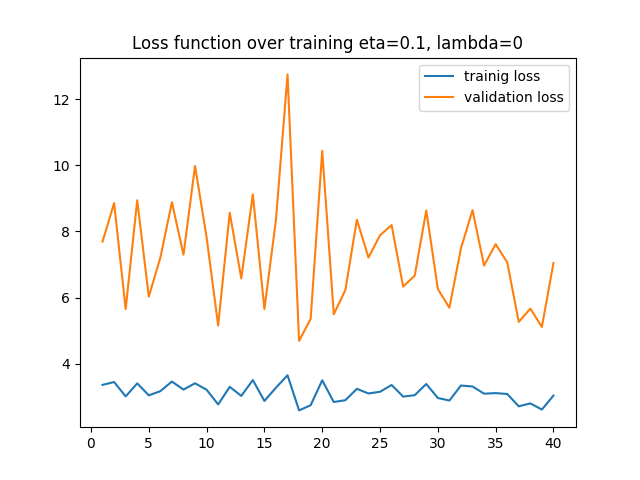
\includegraphics[width=.32\linewidth]{images/loss_over_trainig_eta=0.1_lambda=0.png}
		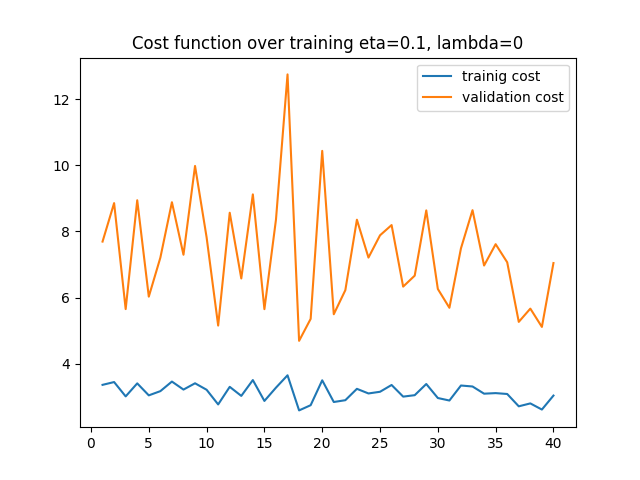
\includegraphics[width=.32\linewidth]{images/cost_over_trainig_eta=0.1_lambda=0.png}
		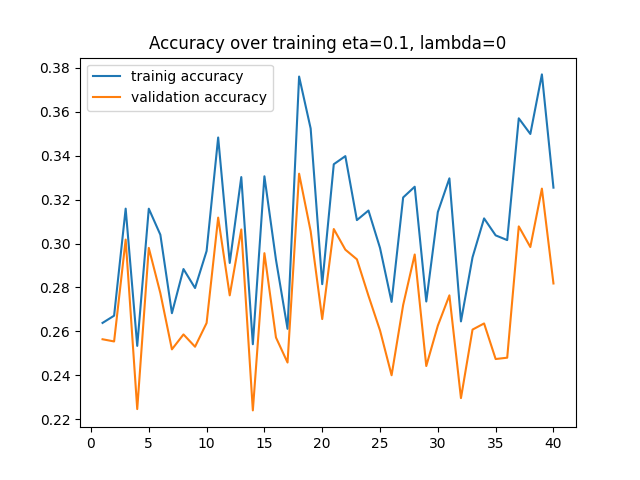
\includegraphics[width=.32\linewidth]{images/accuracy_over_trainig_eta=0.1_lambda=0.png}
		\caption{$\lambda=0, \; \eta = 0.1$ }
	\end{subfigure}

	\begin{subfigure}{\textwidth}
		\centering
		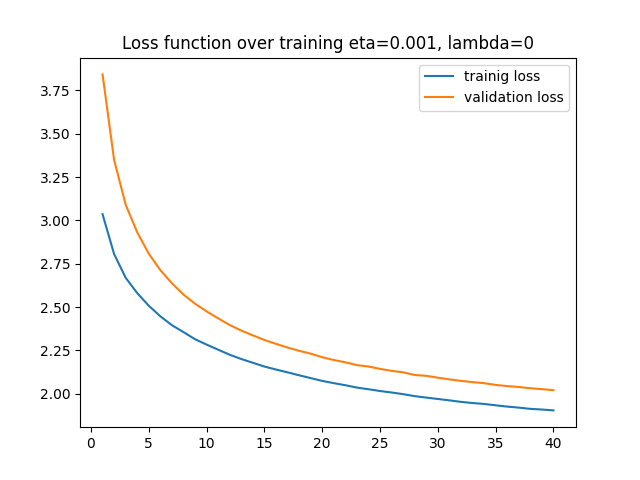
\includegraphics[width=.32\linewidth]{images/loss_over_trainig_eta=0.001_lambda=0.png}
		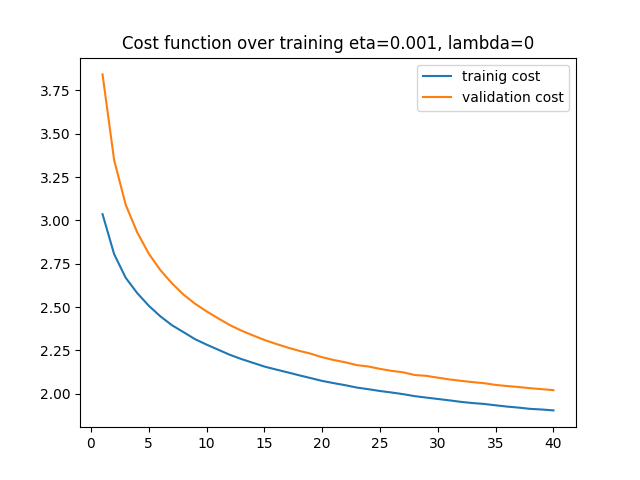
\includegraphics[width=.32\linewidth]{images/cost_over_trainig_eta=0.001_lambda=0.png}
		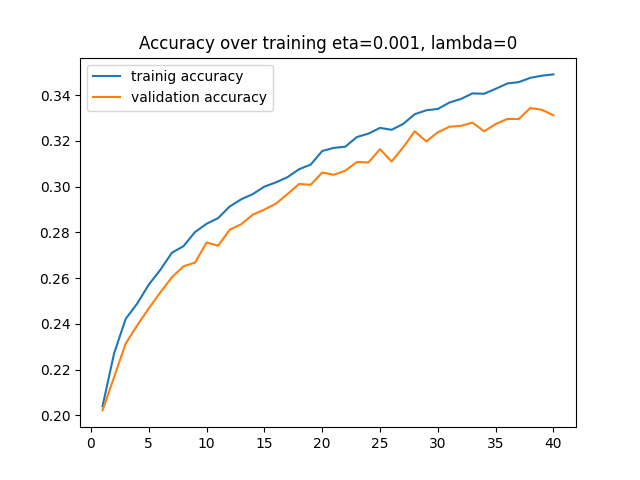
\includegraphics[width=.32\linewidth]{images/accuracy_over_trainig_eta=0.001_lambda=0.png}
		\caption{$\lambda=0, \; \eta = 0.001$ }
	\end{subfigure}

	\begin{subfigure}{\textwidth}
		\centering
		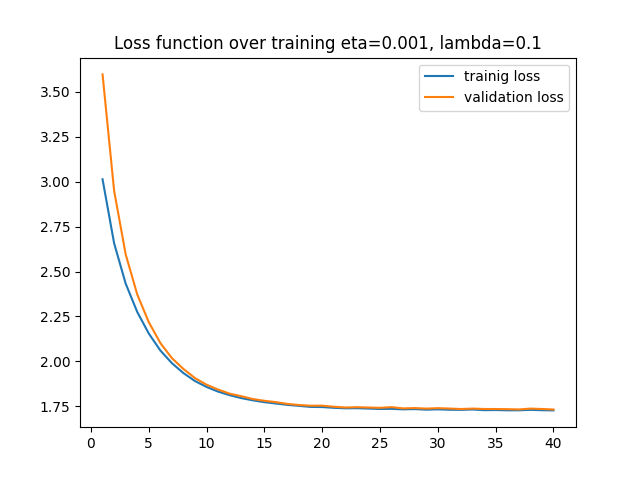
\includegraphics[width=.32\linewidth]{images/loss_over_trainig_eta=0.001_lambda=0.1.png}
		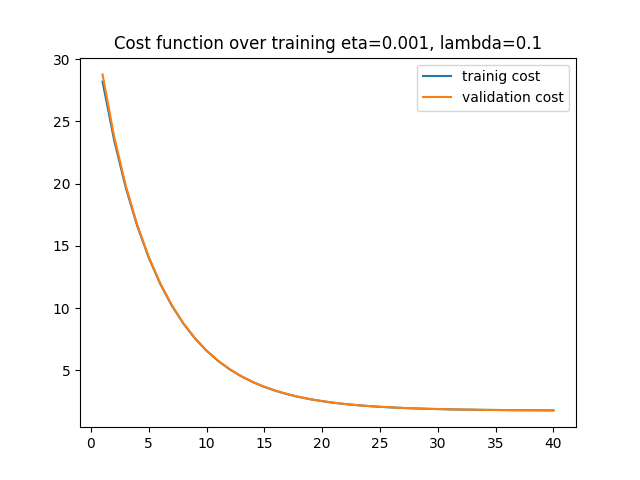
\includegraphics[width=.32\linewidth]{images/cost_over_trainig_eta=0.001_lambda=0.1.png}
		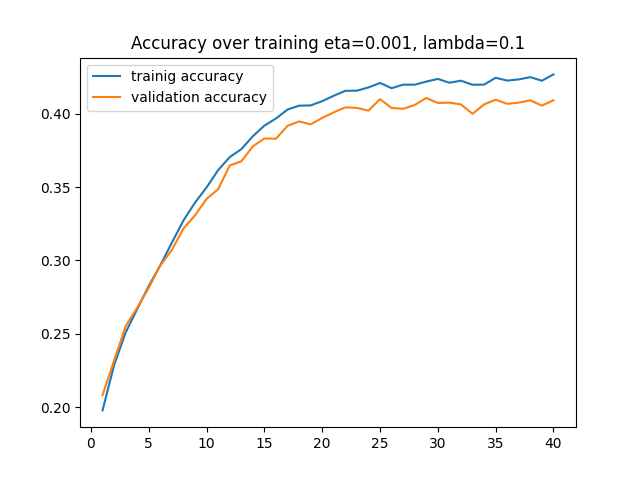
\includegraphics[width=.32\linewidth]{images/accuracy_over_trainig_eta=0.001_lambda=0.1.png}
		\caption{$\lambda=0.1, \; \eta = 0.001$ }
	\end{subfigure}

	\begin{subfigure}{\textwidth}
		\centering
		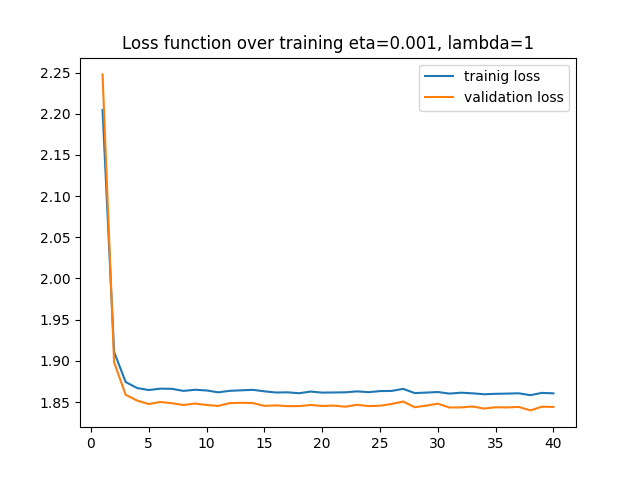
\includegraphics[width=.32\linewidth]{images/loss_over_trainig_eta=0.001_lambda=1.png}
		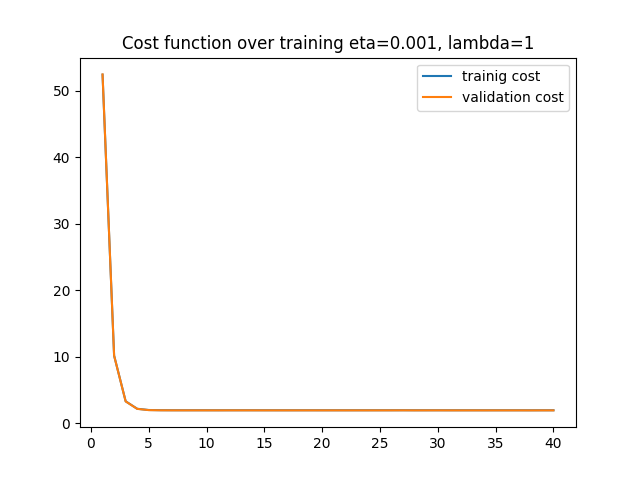
\includegraphics[width=.32\linewidth]{images/cost_over_trainig_eta=0.001_lambda=1.png}
		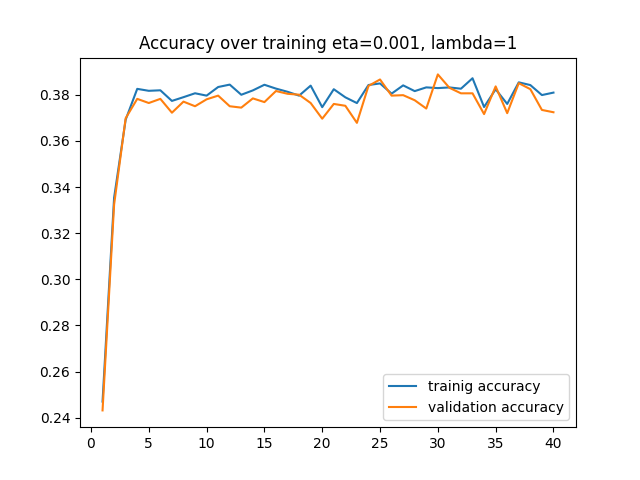
\includegraphics[width=.32\linewidth]{images/accuracy_over_trainig_eta=0.001_lambda=1.png}
		\caption{$\lambda=1, \; \eta = 0.001$ }
	\end{subfigure}

	\caption{Loss, cost and accuracy of the model during training.}
	\label{fig:training}
\end{figure}

We can see that when we set 0.1 as the learning rate, the network reaches a not-so-bad point after the first iteration; however, it keeps overshooting the optimal values and does not converge to a good set of weights. In this setting, the network jumps around, and it does not have adequate performance in the evaluation. However, when we change the learning rate to 0.001, the network converges, and the final accuracy increases. It is worth mentioning that when we do not use regularization ($\lambda=0$), the validation and training loss and accuracy have a considerable difference, and the network's performance is better on training data that it has seen. As expected, when we increase $\lambda$, this difference decreases, and the generalization performance of the network enhances. However, when we have $\lambda = 1$, the network's performance decreases. It may be because this value would enforce a strong constraint on our network, which structure is very simple. So, the network would not be able to optimize the weights to decrease the loss function effectively.

Also, the visualization of the $W$ can be found in \autoref{fig:w_vis}. As we see, by increasing the $\lambda$, we have a smoother matrix. Also, when we do not use regularization, the network does not seem to capture any repetitive pattern in each class, while by using regularization, instead of memorizing the training set, the model learns these patterns.






\begin{figure}[h]
	\centering
	\begin{subfigure}{\textwidth}
		\centering
		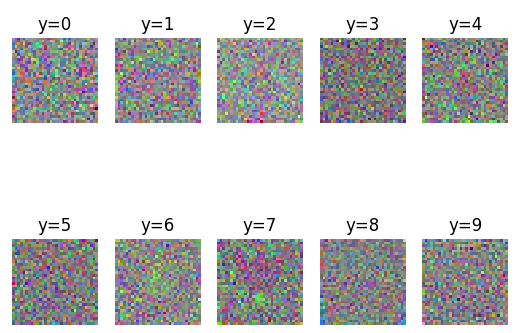
\includegraphics[width=.5\linewidth]{images/weights_eta=0.1_lambda=0.png}
		\caption{$\lambda=0, \; \eta = 0.1$ }
	\end{subfigure}
	
	\begin{subfigure}{\textwidth}
		\centering
		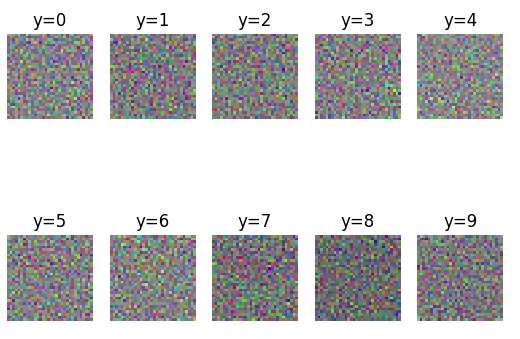
\includegraphics[width=.5\linewidth]{images/weights_eta=0.001_lambda=0.png}
		\caption{$\lambda=0, \; \eta = 0.001$ }
	\end{subfigure}
	
	\begin{subfigure}{\textwidth}
		\centering
		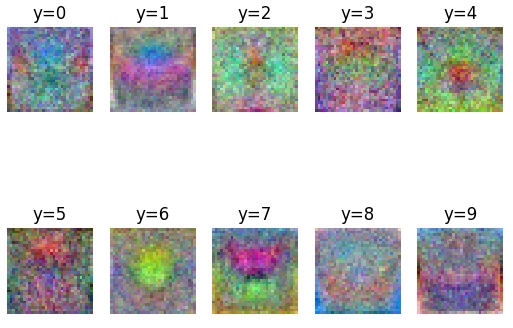
\includegraphics[width=.5\linewidth]{images/weights_eta=0.001_lambda=0.1.png}
		\caption{$\lambda=0.1, \; \eta = 0.001$ }
	\end{subfigure}
	
	\begin{subfigure}{\textwidth}
		\centering
		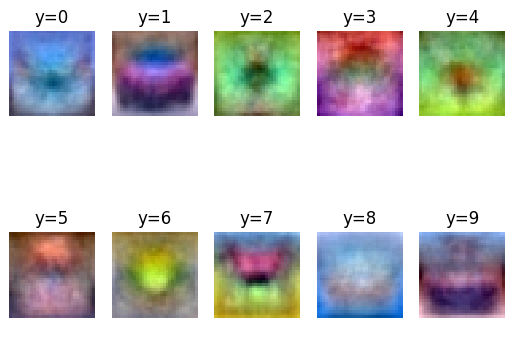
\includegraphics[width=.5\linewidth]{images/weights_eta=0.001_lambda=1.png}
		\caption{$\lambda=1, \; \eta = 0.001$ }
	\end{subfigure}
	
	\caption{Visualization of W after training.}
	\label{fig:w_vis}
\end{figure}


\section{Implementation Documentation}
\label{sec:2}
blabla


%%%%%%%% EXTRA TIPS %%%%%%%%
%% If you want to include an figure
%%\begin{figure}[H]
%%\includegraphics[]{Pendulum.jpg}
%%\caption{Sketch of the pendulum}
%%\label{fig:pendulum}
%%\end{figure}

%% for multiple figures in one fig
%\begin{figure}[h]
%	\centering
%	\begin{subfigure}{\textwidth}
%		\centering
%		\includegraphics[width=\linewidth]{images/sthfivo.png}
%		\caption{}
%	\end{subfigure}
%	\begin{subfigure}{\textwidth}
%		\centering
%		\includegraphics[width=\linewidth]{images/sth.png}
%		\caption{}
%	\end{subfigure}
%	\begin{subfigure}{\textwidth}
%		\centering
%		\includegraphics[width=\linewidth]{images/sth.png}
%		\caption{}
%	\end{subfigure}
%	\caption{caption}
%	\label{fig:label}
%\end{figure}


%% You can then reference with \ref{fig:pendulum}


%%\newpage
\bibliographystyle{apacite}
\bibliography{ref.bib}

\end{document}